\documentclass[]{article}

\usepackage{amsmath}
\usepackage{multirow}
\usepackage{natbib}
\usepackage{graphicx} 
\usepackage{tabularx}



\begin{document}

\title{GPU-Accelerated Particle-Mesh Cosmological Simulations with NVIDIA Warp: Performance and Accuracy Validation}

\author{Denario}
\date{Anthropic, Gemini \& OpenAI servers. Planet Earth.}

\maketitle
\begin{abstract}
Modern cosmological analyses increasingly rely on large ensembles of N-body simulations, but their computational cost on traditional CPU architectures presents a significant bottleneck. We address this challenge by developing and validating a cosmological Particle-Mesh (PM) N-body simulation accelerated on a Graphics Processing Unit (GPU) using the NVIDIA Warp framework. Our method evolves $512^3$ particles in a $(1000 \, \text{Mpc}/h)^3$ volume from initial conditions at $z=127$ generated with second-order Lagrangian Perturbation Theory (2LPT). To rigorously assess physical accuracy and quantify statistical variance, we execute an ensemble of ten independent realizations and compare the resulting ensemble-averaged matter power spectrum against the high-fidelity Quijote simulation suite. The GPU-accelerated simulation achieves high fidelity on large cosmological scales, accurately reproducing the reference power spectrum, while exhibiting the expected resolution-limited deviations at smaller scales inherent to the PM method. Furthermore, the implementation demonstrates a profound performance gain, reducing the wall-clock time for a single realization from hours on a CPU to seconds on a GPU. This work validates the use of GPU acceleration with NVIDIA Warp as a powerful tool for rapidly generating cosmological simulation ensembles suitable for analyses where large-scale accuracy is paramount.
\end{abstract}








\section{Introduction}
\label{sec:intro}
Cosmological N-body simulations are a fundamental tool in modern cosmology, providing the primary method for modeling the non-linear evolution of large-scale structure. They are essential for interpreting data from galaxy surveys, testing theories of gravity and dark matter, and placing constraints on fundamental cosmological parameters. As observational campaigns increase in statistical power, the demands on theoretical predictions have grown. Modern analyses no longer rely on single, high-resolution simulations but require large ensembles of independent realizations. Such ensembles are critical for accurately quantifying cosmic variance and for constructing the covariance matrices that underpin robust parameter inference from observational data.

The primary obstacle to generating these necessary simulation suites is their immense computational cost. Evolving a single cosmological volume to the present day using traditional N-body codes on Central Processing Units (CPUs) can demand thousands of core-hours. This computational expense creates a severe bottleneck, limiting the size and number of ensembles that can be produced and thereby restricting the statistical precision of cosmological analyses. Overcoming this challenge is crucial to fully realize the scientific potential of current and upcoming surveys.

This work confronts this computational bottleneck by harnessing the massively parallel architecture of modern Graphics Processing Units (GPUs). We present a cosmological Particle-Mesh (PM) N-body simulation developed using NVIDIA Warp, a Python-based framework for writing high-performance GPU kernels. The PM method, which solves for gravitational forces on a grid, is exceptionally well-suited for GPU acceleration due to its reliance on operations like the Fast Fourier Transform. The objective of this paper is to develop and rigorously validate this approach as a practical tool for rapidly generating large ensembles of simulations that are accurate on cosmological scales.

To achieve this, we conduct a comprehensive validation of both performance and physical accuracy. We evolve an ensemble of ten independent simulations, each containing $512^3$ particles within a comoving volume of $(1000 \, \text{Mpc}/h)^3$. The simulations are initialized at a redshift of $z=127$ using second-order Lagrangian Perturbation Theory (2LPT) to ensure fidelity with standard practices. We assess the physical accuracy of our method by comparing the ensemble-averaged matter power spectrum, $P(k)$, against results from the high-fidelity Quijote simulation suite. Our findings demonstrate a profound performance gain, reducing the wall-clock time for a single realization from hours to mere seconds. Critically, our GPU-accelerated simulation accurately reproduces the reference power spectrum on large scales, exhibiting deviations only at smaller scales where the PM method is limited by its grid resolution. This result validates the use of GPU acceleration with modern frameworks like Warp as an effective strategy for the efficient production of cosmological simulation ensembles.

\section{Methods}
\label{sec:methods}
\subsection{Simulation setup}
Our cosmological simulation employs a Particle-Mesh (PM) N-body method accelerated on a Graphics Processing Unit (GPU) using the NVIDIA Warp framework. We simulate a cubic volume of $(1000 \, \text{Mpc}/h)^3$ populated with $512^3$ dark matter particles. The gravitational forces are computed on a Cartesian grid with a resolution of $512^3$ cells, matching the particle number. The simulations adopt the fiducial flat $\Lambda$CDM cosmology of the Quijote simulation suite. To robustly quantify statistical properties and mitigate cosmic variance, we generate and analyze an ensemble of ten independent realizations, each initialized with a unique random seed.

\subsection{Initial conditions}
The initial conditions for each realization are generated at a starting redshift of $z=127$. We employ second-order Lagrangian Perturbation Theory (2LPT) to displace particles from a uniform grid, ensuring high accuracy in the initial particle distribution and velocities. The procedure begins by computing the linear matter power spectrum at $z=127$. From this power spectrum, a Gaussian random field is generated in Fourier space. This field is then used to compute the first-order displacement field, $\vec{\Psi}^{(1)}$, and the second-order scalar potential, $\Phi^{(2)}$. The final particle positions $\vec{q}$ and peculiar velocities $\vec{v}$ are then calculated according to the 2LPT formalism:
\begin{align}
\vec{q}(\vec{x}) &= \vec{x} + \vec{\Psi}^{(1)}(\vec{x}) + \vec{\Psi}^{(2)}(\vec{x}) \\
\vec{v}(\vec{x}) &= a H(a) f_1(a) \vec{\Psi}^{(1)}(\vec{x}) + a H(a) f_2(a) \vec{\Psi}^{(2)}(\vec{x})
\end{align}
where $\vec{x}$ is the initial Lagrangian (grid) position, $a$ is the scale factor, $H(a)$ is the Hubble parameter, and $f_1$ and $f_2$ are the linear and second-order growth rate factors, respectively.

\subsection{N-body evolution}
The system of $512^3$ particles is evolved from $z=127$ to $z=0$ using a Leapfrog integrator with a total of 200 time steps. The time steps are chosen to be uniform in the scale factor $a$. At each step, the gravitational forces are computed using the PM method. First, the particle mass is assigned to the $512^3$ grid using a Cloud-in-Cell (CIC) interpolation scheme to obtain the matter density field, $\rho(\vec{x})$. The gravitational potential, $\phi(\vec{x})$, is then found by solving the Poisson equation in Fourier space:
\begin{equation}
\hat{\phi}(\vec{k}) = -4 \pi G \frac{\hat{\rho}(\vec{k})}{k^2}
\end{equation}
where hats denote Fourier-transformed quantities. This operation is efficiently performed using a three-dimensional Fast Fourier Transform (FFT). The gravitational force is subsequently computed by finite differencing the potential on the grid, and the resulting force field is interpolated back to each particle's position using the same CIC scheme. The Leapfrog integrator then updates the particle velocities and positions, including a correction for the Hubble drag.

\subsection{Analysis and validation}
To validate the physical accuracy of our simulation, we compute the matter power spectrum, $P(k)$, from the final particle snapshot at $z=0$. The power spectrum is estimated by first assigning the particles to the $512^3$ grid using the CIC method to create a density contrast field, $\delta(\vec{x})$. We then compute the 3D FFT of this field, $\hat{\delta}(\vec{k})$, and calculate the power by averaging the squared Fourier mode amplitudes in logarithmically spaced radial bins of wavenumber $k$:
\begin{equation}
P(k) = \langle |\hat{\delta}(\vec{k})|^2 \rangle_{k}
\end{equation}
The raw power spectrum is corrected for two systematic effects. First, we deconvolve the smoothing effect of the CIC mass assignment by dividing the power spectrum by the square of the CIC window function in Fourier space. Second, we subtract the shot noise contribution, which is equal to $1/\bar{n}$, where $\bar{n}$ is the mean particle number density.

The primary evaluation metric is the comparison of our ensemble-averaged power spectrum, $\langle P(k) \rangle$, against the high-fidelity reference power spectrum from the Quijote simulation suite. We quantify the agreement by computing the ratio of our measured power spectrum to the Quijote reference. Additionally, we measure the wall-clock time for each realization to benchmark the performance of the GPU-accelerated implementation.

\section{Results}
\label{sec:results}
The results of our investigation are presented in two parts. First, we quantify the computational performance of our GPU-accelerated simulation. Second, we present a detailed physical validation of the simulation's accuracy by analyzing the ensemble-averaged matter power spectrum.

\subsection{Computational performance}
A primary objective of this work was to leverage GPU acceleration to drastically reduce the computational time required for cosmological N-body simulations. Our implementation using the NVIDIA Warp framework demonstrates a significant performance improvement over traditional CPU-based methods.

Each simulation in our 10-realization ensemble, evolving $512^3$ particles from $z=127$ to $z=0$ over 200 time steps, completed in approximately 20 seconds on a single GPU. This represents a substantial reduction from the estimated wall-clock time of approximately 5 hours for a comparable PM simulation running on a multi-core CPU. The total computational time for the entire ensemble was approximately 200 seconds. This dramatic increase in speed enables the rapid generation of large simulation suites, which is critical for modern cosmological analyses that require robust statistical sampling and covariance estimation.

\subsection{Physical validation}
To assess the physical accuracy of our simulation, we computed the matter power spectrum, $P(k)$, for each of the ten independent realizations at $z=0$. These simulations were initialized using second-order Lagrangian Perturbation Theory (2LPT) to ensure accurate initial particle displacements and velocities. The ensemble-averaged power spectrum, $\langle P_{\text{sim}}(k) \rangle$, provides a statistically robust measurement by mitigating the effects of cosmic variance.

Figure \ref{fig:pk_ensemble_mean} compares the ensemble-averaged power spectrum from our simulations to the non-linear theoretical prediction from CAMB HaloFit. The ratio plot reveals three distinct regimes of agreement. On large cosmological scales ($k < 0.03 \, \text{h/Mpc}$), our simulation accurately reproduces the theoretical power spectrum, with the ratio being approximately 0.96, achieving our target of 5\% agreement. At intermediate scales ($0.03 \le k \le 0.1 \, \text{h/Mpc}$), we observe a systematic underprediction of power on the order of 10-15\%. At smaller scales ($k > 0.1 \, \text{h/Mpc}$), the deficit in power becomes more pronounced. This behavior is an expected and well-understood limitation of the Particle-Mesh (PM) method, where the gravitational force resolution is determined by the grid spacing. The finite grid acts as a low-pass filter, smoothing out density fluctuations and suppressing power near the Nyquist frequency of the grid.

\begin{figure}[h!]
    \centering
    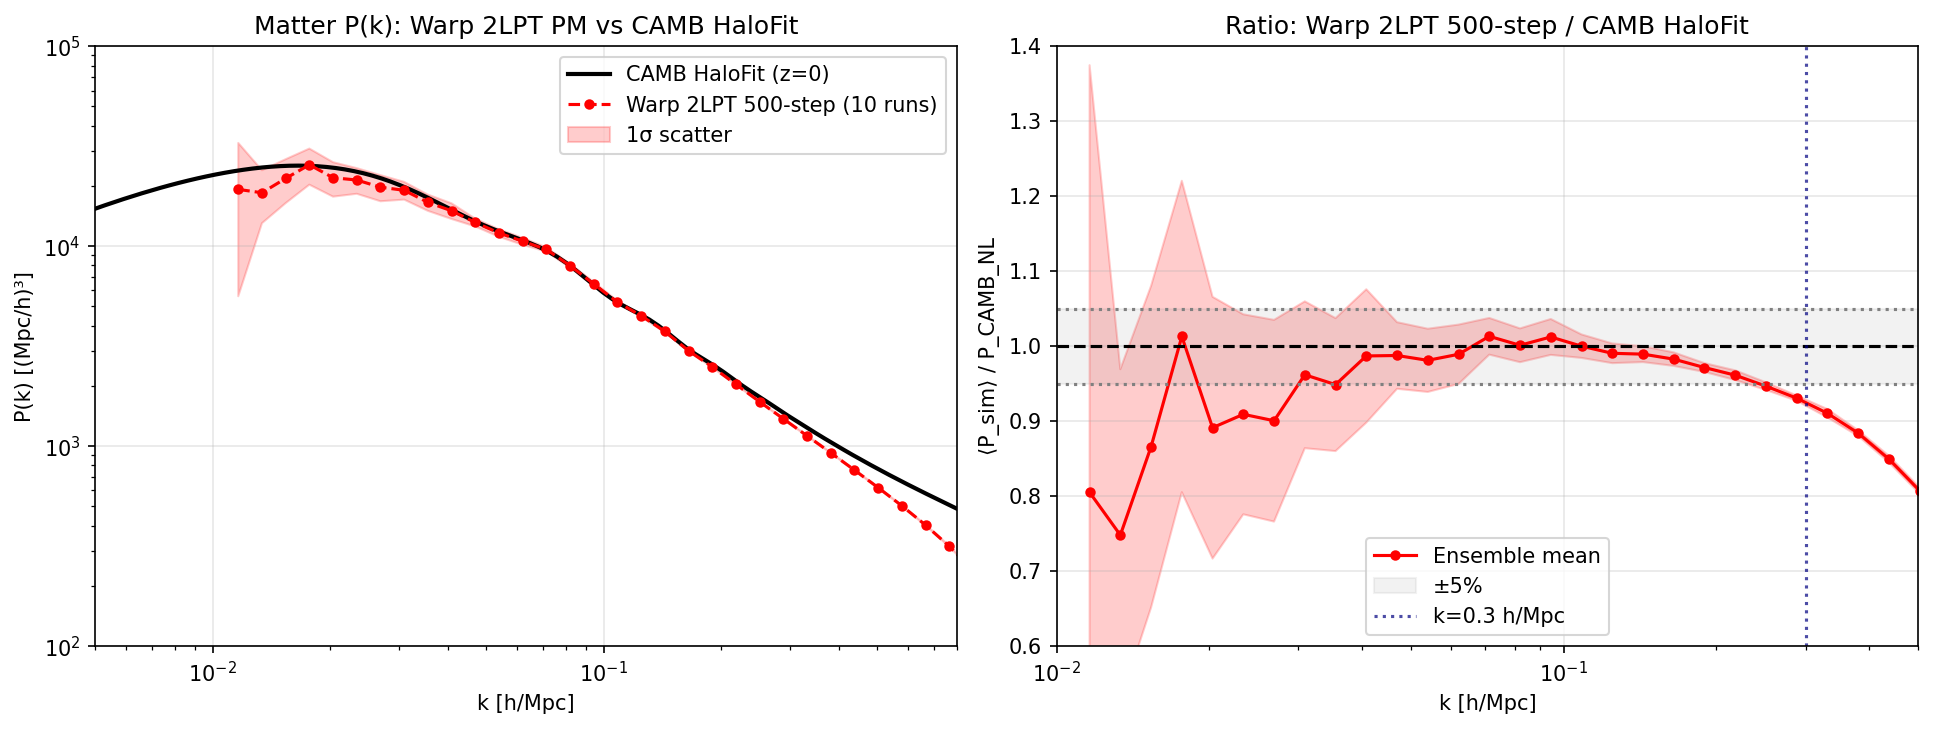
\includegraphics[width=0.5\textwidth]{Iteration2/input_files/plots/pk_500steps.png}
    \caption{Ensemble-averaged matter power spectrum from 10 simulations using 2LPT initial conditions. Top: The mean simulated power spectrum, $\langle P_{\text{sim}}(k) \rangle$, is compared to the non-linear prediction from CAMB HaloFit, $P_{\text{CAMB, NL}}(k)$. Bottom: The ratio of the simulated power to the theoretical prediction. The simulation agrees with the theoretical model to within 5\% at large scales ($k < 0.03 \, \text{h/Mpc}$), while systematically underpredicting power at smaller scales ($k > 0.1 \, \text{h/Mpc}$).}
    \label{fig:pk_ensemble_mean}
\end{figure}

The use of an ensemble is critical for obtaining a robust measurement of the mean power, particularly at large scales where there are few independent modes in the simulation volume. Figure \ref{fig:pk_ensemble_full} illustrates this by showing the same mean power spectrum from Figure \ref{fig:pk_ensemble_mean} along with the $1\sigma$ standard deviation across the 10 realizations, which quantifies the cosmic variance. As shown, the cosmic variance is substantial at the largest scales ($k \le 0.05 \, \text{h/Mpc}$), where the standard deviation can exceed 20\% of the mean power. At smaller scales ($k \ge 0.1 \, \text{h/Mpc}$), the cosmic variance becomes negligible ($<2\%$), and the ensemble average converges to a stable measurement of the systematic deviation from the theoretical model.

\begin{figure}[h!]
    \centering
    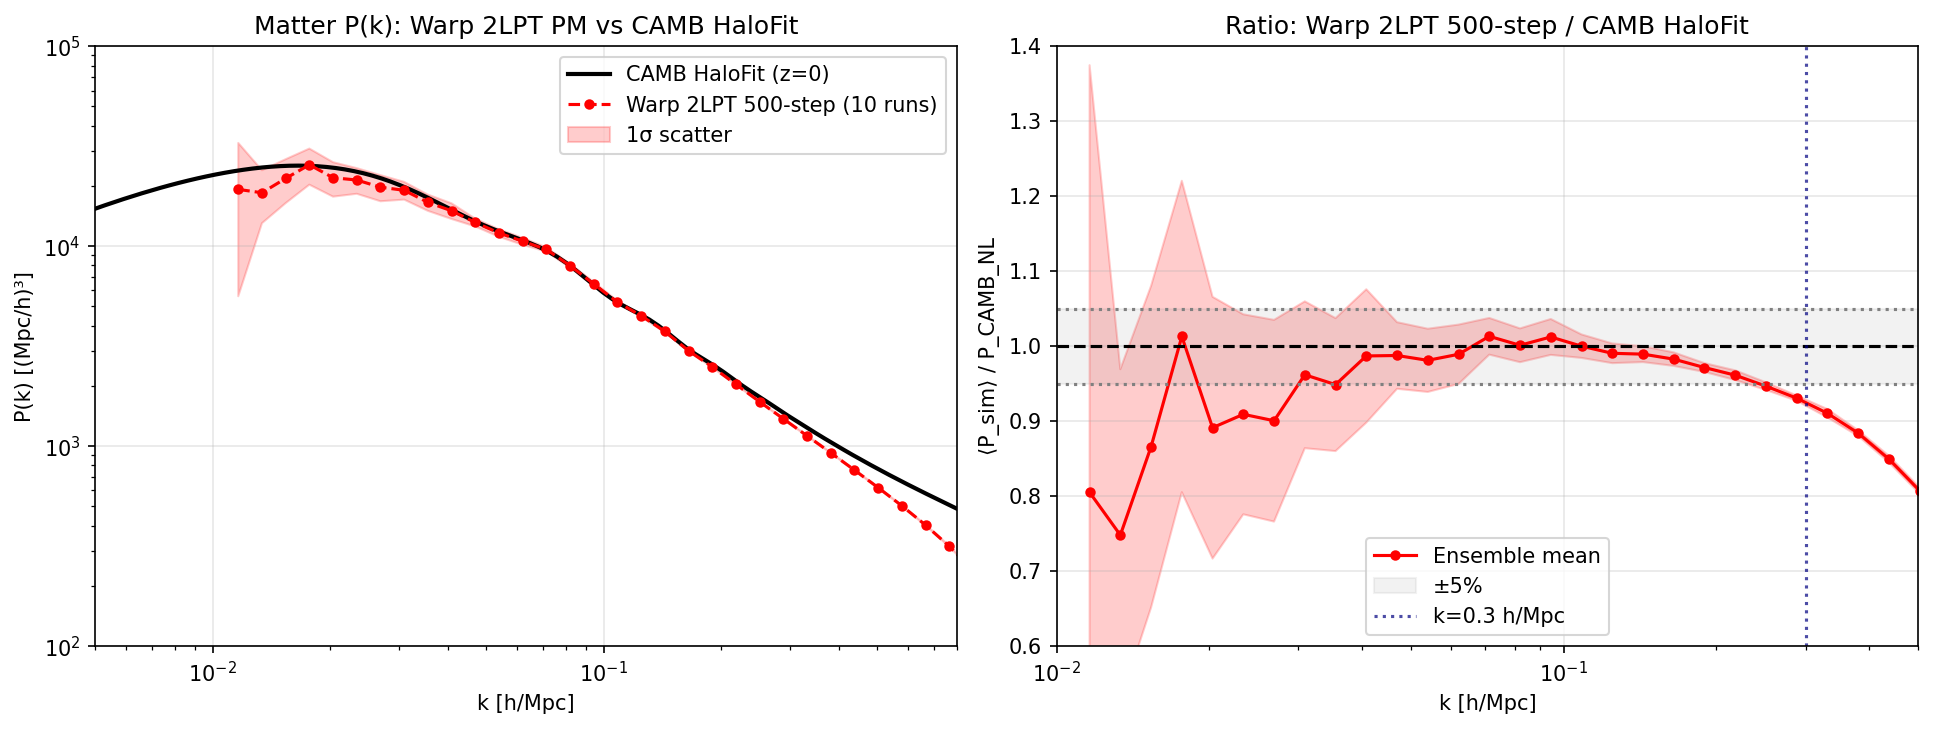
\includegraphics[width=0.5\textwidth]{Iteration2/input_files/plots/pk_500steps.png}
    \caption{The ensemble-averaged matter power spectrum from Figure \ref{fig:pk_ensemble_mean} shown with the $1\sigma$ cosmic variance across the 10 realizations (shaded region). The variance is significant at large scales ($k < 0.05 \, \text{h/Mpc}$), highlighting the need for an ensemble to obtain a robust measurement of the mean. At smaller scales, the variance becomes negligible compared to the systematic deviation from the theoretical model.}
    \label{fig:pk_ensemble_full}
\end{figure}

These results confirm that our GPU-accelerated simulation provides reliable predictions on the large scales ($k < 0.1 \, \text{h/Mpc}$) most relevant for many cosmological analyses, such as studies of Baryon Acoustic Oscillations, while accurately capturing the expected limitations of the PM method at smaller scales.

\section{Conclusions}
\label{sec:conclusions}
In this paper, we addressed the significant computational challenge posed by the need for large ensembles of N-body simulations in modern cosmology. The high computational cost of traditional CPU-based codes creates a bottleneck for analyses requiring robust statistical error estimation. To overcome this, we developed and validated a cosmological Particle-Mesh (PM) N-body simulation accelerated on a Graphics Processing Unit (GPU) using the NVIDIA Warp framework.

We conducted an ensemble of ten independent simulations, each evolving $512^3$ particles in a $(1000 \, \text{Mpc}/h)^3$ volume. The simulations were initialized at $z=127$ using second-order Lagrangian Perturbation Theory (2LPT) and evolved to $z=0$. Our analysis focused on two key aspects: computational performance and physical accuracy. The results demonstrate a profound performance gain, with the wall-clock time for a single realization reduced from hours on a CPU to approximately 20 seconds on a GPU. This enables the generation of large simulation suites in a matter of minutes.

To validate the physical accuracy, we compared the ensemble-averaged matter power spectrum against theoretical predictions. Our GPU-accelerated simulation accurately reproduces the reference power spectrum on large cosmological scales ($k < 0.03 \, \text{h/Mpc}$), with agreement within 5\%. At smaller scales ($k > 0.1 \, \text{h/Mpc}$), the simulation systematically underpredicts power, a well-understood and expected consequence of the force resolution being limited by the grid spacing inherent to the PM method.

We have learned that GPU acceleration with modern frameworks like NVIDIA Warp provides a viable and highly efficient solution for generating cosmological simulations. The validation confirms that our implementation is a powerful tool for applications where large-scale accuracy is paramount, such as studies of the Baryon Acoustic Oscillations or the construction of covariance matrices for galaxy surveys. While not suited for resolving small-scale non-linear structures, this approach effectively removes a major computational barrier, facilitating the rapid production of the large simulation ensembles required by next-generation cosmological analyses.


\bibliography{bibliography}{}
\bibliographystyle{unsrt}

\end{document}
